\chapter{Direct light-induced spin transfer between elemental sublattices in a spintronic Heusler material via femtosecond laser excitation}
\label{heuslerpaper}

\section{Introduction}
In this chapter, we move to studying a more complex material, half-metal heusler compound C$o_2$MnGe, using the same tools as previously: time-resolved transverse magneto optical Kerr effect. We show that a single ultrafast laser pulse can directly transfer spin polarization from one magnetic sublattice to another within the duration of the laser excitation pulse. Using the unique ability of extreme ultraviolet high harmonic light resonant at the 3p edges of cobalt and manganese to measure the magnetization of each element simultaneously and independently, we observe a surprising disparity between the response of the two magnetic sublattices: the magnetization of cobalt is transiently enhanced during the laser pump pulse, while that of manganese quenches rapidly. This extremely fast enhancement of the average magnetization of Co represents the fastest change in magnetization observed to date and is a unique property that stems from the half-metallic nature of the Heusler material. 

Next, we use density functional theory (DFT) calculations \cite{Hohenberg1964,KOHN1965}, that compute the density of states for each element in the compound, to show that optical excitations are preferentially enhanced in the majority spin channel of Mn and in the minority spin channel of Co. This imbalance of allowed excitation pathways for each element then induces a direct and instantaneous transfer of spin polarization from Mn sites to Co sites that occurs during the entire duration of the laser pulse. As a control, we observe no enhancement of magnetization or transfer of spin polarization in the disordered non-half-metallic (A2) phase of the same material. This is consistent with electronic structure theory that does not support any imbalance in the excited spin population of manganese in this phase. The observed transient enhancement of ferromagnetic ordering demonstrates direct manipulation of spins via light, thus providing a path towards spintronic logic devices such as switches that can operate on few femtosecond or even faster timescales. It also establishes band structure engineering as an efficient method of selecting for specific desirable behaviors in a quantum material.

\begin{figure}
\label{fig: Heus1}
\begin{center}
	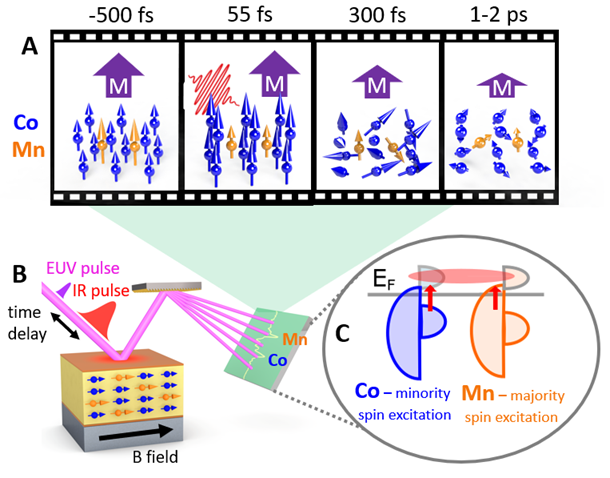
\includegraphics[width=150mm]{figs/Heus1}
\end{center}
\caption{(A) Representation of spin dynamics in C$o_2$MnGe. Before excitation, Mn atoms (orange arrows) have a 3x larger magnetic moment than Co atoms (blue arrows), which are 2x more abundant in the bcc lattice. The purple arrow represents the net magnetic moment of the compound. Upon excitation, the Mn moment begins to decrease and the Co magnetic moment immediately grows by 10\%. This occurs within the duration of the pump pulse. Hundreds of femtoseconds later, the Mn and Co atomic spins become disordered, and the angular momentum begins to transfer to the lattice. The net magnetic moment begins to decrease. After 1-2 ps, the spins have reached their maximum quenching. (B) Schematic of the experimental apparatus. Ultrafast femtosecond infrared pulses are used to excite the sample, while the magnetization dynamics are tracked with femtosecond EUV pulses recorded on a spectrometer. (C) Density of states for each element in the half metal. Note that the minority spin channel is gapped, with no available states at the Fermi level for the minority channel. Critically, this gap is larger for Mn than for Co. After excitation, the conductions band states are hybridized, as illustrated by the shared red wavefunction.}
\end{figure}

Figure \ref{fig: Heus1}A illustrates the ultrafast spin dynamics that occur in the B2 (semi-ordered) half-metallic phase of C$o_2$MnGe. Before the pump pulse arrives, the material is ferromagnetically ordered, with a B2 structure (the CsCl structure), where Co occupies the corner sites, and the body centered position is randomly occupied by Mn or Ge. Note that the Mn atoms carry $\approx$3x as much magnetic moment as the Co atoms. As shown in Figs. 1 and 2, within the timescale of the laser pump pulse, there is a direct transfer of magnetization from the Mn atoms to the Co atoms: the magnetization of the Mn atoms decreases, while the magnetic moment of the Co atoms increases. After the pump pulse, the material continues to demagnetize, dissipating the angular momentum into the lattice within a ps, with a $\approx$120 fs lag between the response of Mn and Co. We emphasize that the initial magnetic response of the system is completely dominated by a direct optical excitation process, while rotation of atomic magnetic moments enters at a second stage. This is corroborated by a theoretical analysis based on the atomistic Landau-Lifshitz-Gilbert equation \cite{Ericksson2017} (presented in the supplementary information), that fails to describe the initial phase of the magnetic response ($<$ 250 ps) but provides the correct trend for longer time scales ($>$500 fs).

\section{Experimental Results}
Figure \ref{fig: Heus1}B shows the experimental setup used to simultaneously measure the response of Co and Mn after ultrafast excitation. We excite the sample with an infrared laser pulse with a photon energy of 1.55 eV and 55 fs full width half maximum (FWHM) in duration. To record the magnetic response, part of the laser light is directed into a He-filled hollow waveguide to generate 10 fs high harmonic EUV pulses that are simultaneously resonant with the 3p edges of Co (59 eV) and Mn (47 eV). The EUV transverse magneto optical Kerr effect (TMOKE) signal is constructed by a differential asymmetry [A] measurement with A=$\frac{I_+ - I_-}{I_+ + I_-}$ where $I_+$ and $I_-$ are the intensities of the EUV light that is reflected from the sample for opposite directions of magnetization. The responses from individual elements are separated via a spectrometer. A more detailed schematic of the experimental layout is given later in the chapter.

\begin{figure}
	\label{fig: Heus2}
	\begin{center}
		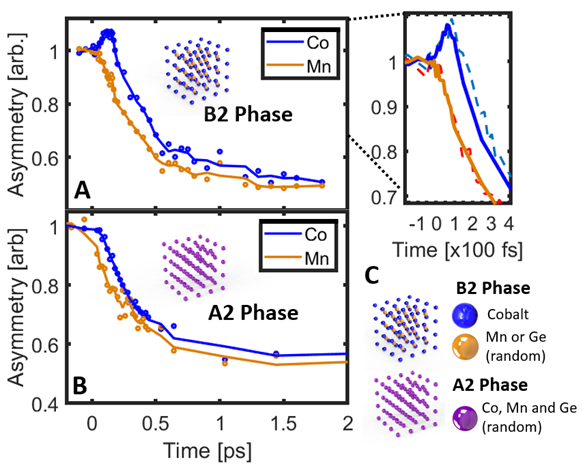
\includegraphics[width=150mm]{figs/Heus2}
	\end{center}
	\caption{Element resolved ultrafast magnetization dynamics following excitation by femtosecond laser in the (A) half-metallic B2 phase. Note that the Co magnetization increases as the Mn decreases, followed by a lag of ~100 fs between the demagnetization of the Co and Mn sublattices. Inset: Dynamics of ultrafast spin transfer. Solid lines are the element specific dynamics after excitation by a 55 fs (full width half maximum) pump pulse. Dashed lines indicate the dynamics after excitation by a 90 fs pump pulse. Note that the location of the peak of the enhancement is shifted in time by ~25 fs for the enhancement driven by a 90 fs pump (half the difference between the duration of the two pulses), underlining that this process is a direct optical manipulation. (B) Element resolved ultrafast magnetization dynamics in the non half-metallic A2 phase. There is no enhancement of the Co magnetization. The subsequent lag in demagnetization dynamics between the Co and Mn sublattices decreases to 57 fs. (C) Atomic structure of compounds studied. In the B2 phase, the Co atoms have ordered so that they occupy sites at the edges of the bcc structure, while the centers are randomly interspersed between Mn and Ge. In the A2 phase, the material has formed the ordered bcc structure, but the location of the atoms within the structure are random.}
\end{figure}

Figure \ref{fig: Heus2}A plots the experimentally measured asymmetry of Co and Mn in the half-metallic B2 phase as a function of pump probe time delay. During the laser pulse, the Co magnetization transiently increases by $\approx$ 10\%, while that of Mn immediately decreases. Although the initial dynamics are markedly different, the decay rates of the two magnetic sublattices are similar, and occur on timescales similar to the average values measured by visible MOKE \cite{Mann2012}: Mn demagnetizes with an exponential decay constant of 328 $\pm$ 37 fs while Co does so with a decay constant of  323 $\pm$ 86 fs (after a lag due to the initial transient enhancement). As the timescale for this process is longer than in pure ferromagnets (see SI), we can unambiguously decouple the direct optically generated spin dynamics (that occur over the entire laser pulse duration of 55 fs) from the dissipation of angular momentum in the system (that follows in the next ps). As yet another control to test the time sequence of spin transfer, we increased the pump pulse duration from 55 fs to 90 fs. As shown in dashed lines in the inset of Fig. 2A, this resulted in an increase of the delay in the demagnetization between the Co and Mn sublattices: from 120 $\pm$ 33 fs (55 fs pump pulse) to 157 $\pm$ 27 fs (90 fs pump pulse). This is consistent with a spin transfer process from Mn to Co that occurs only during the laser pump pulse.

Figure \ref{fig: Heus2}B plots the element specific dynamics in the metallic A2 phase of the material driven by a 90 fs excitation pulse. In this phase, the lag in response of the magnetic sublattices (Mn and Co) is much less, only 56 $\pm$ 32 fs, and no transient increase in the Co magnetization is observed. As discussed below and in the SI, this is because the optical pathways to excitation in the minority band of manganese is not blocked in this phase. Fig. \ref{fig: Heus2}C shows the elemental crystal structure of the material in the two phases studied (B2 and A2). The details of sample growth are given in \ref{Shaw2018}. In contrast to the B2 phase, the A2 phase is disordered, does not have a half-metallic gap for the minority spin state (as shown in Fig. 3B), and serves as a control from which to understand the effect of half-metallicity on the element specific magnetization properties of C$o_2$MnGe.

It is clear from a comparison between the dynamics observed in the A2 and B2 phases that ordering and emergence of a half-metallic gap in the minority band play a fundamental role in the optical magnetic response of C$o_2$MnGe. The transient enhancement observed is a coherent process driven directly by the optical excitation pulse, as demonstrated by the shift in the peak of the Co excitation when driven by a longer laser pulse. Moreover, our measurements also show that elemental specificity is critical for revealing the underlying magnetic dynamics of this material: as shown in Fig. \ref{fig: Heus2} and the SI, when the Co and Mn responses are averaged (as is the case for visible MOKE), no difference in the behavior of the A2 and B2 phases can be detected. 

\section{Computational Results}
Figures \ref{fig: Heus3}A and B plot the element specific spin resolved density of states (DOS) calculated using DFT for the two phases of the material. In the B2 phase (Fig. \ref{fig: Heus3}A) a gap has formed for the minority carriers, while the majority has full mobility across the Fermi level. Critically, this gap is larger for the Mn states than the Co states. In contrast, the crystal has a fully metallic characteristic in the A2 phase (Fig. \ref{fig: Heus3}B) for both the majority and minority states. When a 1.55 eV IR photon is absorbed, the density of states of each phase results in several key differences in the transition probabilities for the material. As shown in Fig. \ref*{fig: Heus4} and the SI, in the B2 phase, most of the minority carriers that are excited come from Co states, but very few minority excitations can take place for Mn states. One must bear in mind that both initial and final states of this optical excitation involve wavefunctions that are shared across hybridizing Mn and Co orbitals. Due to an imbalance in how Co and Mn projected orbitals contribute to the initial and final states, direct and spin conserving transitions lead to an effective transfer of spin angular momentum from Mn to Co. 

\begin{figure}
	\label{fig: Heus3}
	\begin{center}
		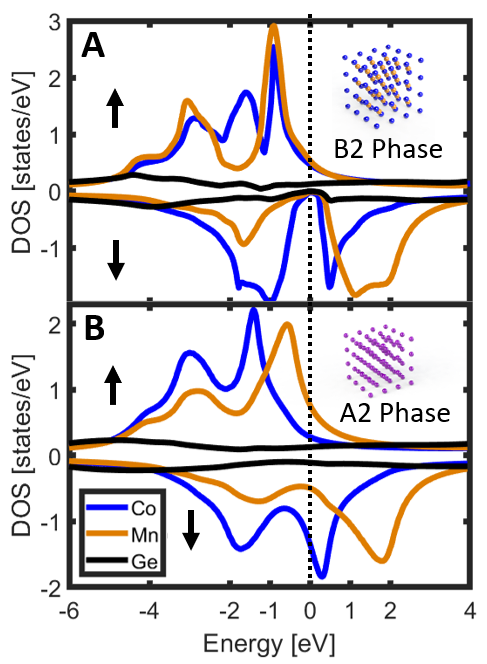
\includegraphics[width=80mm]{figs/Heus3}
	\end{center}
	\caption{Density of states for Co2MnGe in the (A) B2 and (B) A2 phases. Note that the half-metallic character is only present in the B2 phase. }
\end{figure}

Figures \ref{fig: Heus4}A and B plot the calculated imbalance of the transition probabilities from each sublattice that give rise to the spin transfer from Mn to Co. The combination of these effects results in a direct transfer of spin polarization from Mn sublattices to Co as observed experimentally in the B2 phase and illustrated in Fig. 1C. In Fig. \ref{fig: Heus4}C, we illustrate the basic mechanism that allows for an effective angular momentum transfer from Mn d-states to Co d-states. The initial state wavefunction that is involved in the optical transition is hybridized and composed of both Mn and Co d-states, with a larger contribution from the Mn atom (initial state). For the final state, the situation is reversed, and the Co d-states dominate. Hence, when an electron is optically excited from the initial to the final state wavefunction, this is associated with a transfer of d-state population from Mn to Co. A higher probability of transitions for the spin-up electrons compared to the spin-down electrons in Mn (Fig. \ref*{fig: Heus4}A) then causes an effective spin-transfer from Mn to Co, as observed in the data of Fig. \ref{fig: Heus2}A. In the A2 phase (Fig. \ref{fig: Heus2}B), excitation in the minority valence band of Mn is now optically allowed, and direct optical transfer of spin polarization does not occur (see SI for these calculations).

\begin{figure}
	\label{fig: Heus4}
	\begin{center}
		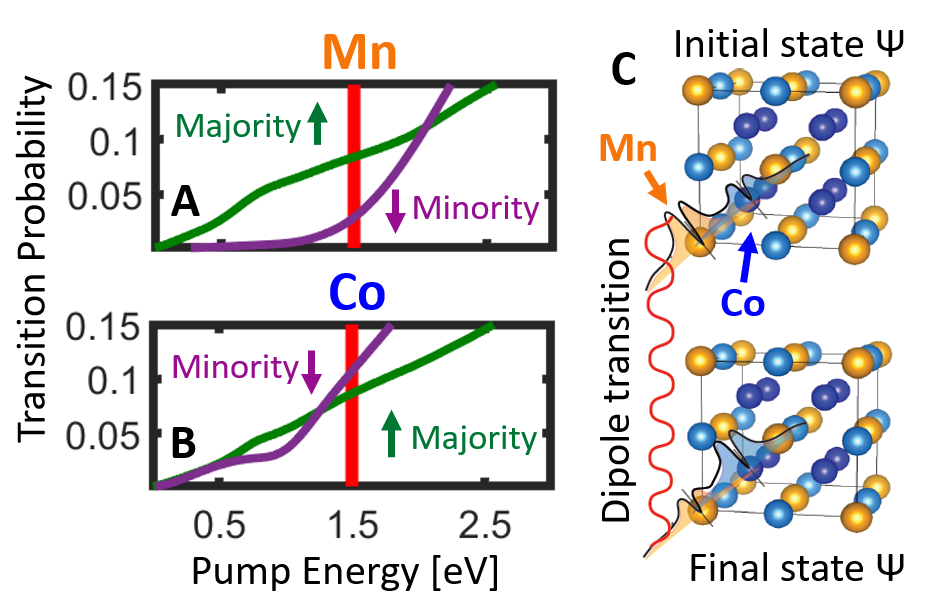
\includegraphics[width=150mm]{figs/Heus4}
	\end{center}
	\caption{The probability for exciting a spin up (majority) vs. spin down (minority) electron from the valence band in the B2 phase for different pump energies in (A) Mn sites. Note that for a 1.55 eV pump, the probability is higher for spin up electrons to be excited from Mn. (B) Probability for excitations in Co sites. In contrast to the Mn result, the probability is higher for minority electrons to be excited in Co. (C) Illustration of process that leads to direct optical transfer of spin polarization from Mn to Co. The initial state wavefunction is hybridized and composed of both Mn and Co d-states, with a larger contribution from the Mn atom. In the final state, the situation is reversed, and the Co d-states dominate. Hence, when an electron is optically excited from the initial to the final state wavefunction, this is associated with a transfer of spin polarization from Mn to Co. }
\end{figure}

We emphasize that the transient enhancement of the magnetic signal shown in Fig. \ref{fig: Heus2}A for the B2 phase has no contribution from the change in refractive index due to electronic changes in the reflectivity. We demonstrate this by measuring the change in reflectivity for the B2 and A2 phases at the Co edge, and showing that the magnitude of these changes is equal in the two phases of the material (see SI for more information). The mechanism responsible for the magnetization dynamics of C$o_2$MnGe in the B2 phase involves direct optical transitions, that leads to an initial transfer of spin moment from Mn to Co. This purely electronic mechanism is necessary in addition to a description based on the atomistic Landau-Lifshitz-Gilbert (aLLG) equation, that sometimes is employed to analyze the kind of experiments presented here \cite{Evans2015,Hofherr2018}. As shown in the SI, the aLLG equation captures some features of the observed magnetization dynamics, especially at longer timescales ($\approx$250 fs and longer), but it fails to explain the initial phase of the demagnetization process. We also note that a similar enhancement to that shown in Fig. $\ref{fig: Heus2}$A was predicted via time dependent DFT calculations for the related compound C$o_2$MnSi, with the mechanism in this case also attributed a transfer of spin polarization between  Co and Mn\cite{Elliott2016}.

\section{Discussion}
Given that we now understand how to measure and predict all-optical spin transfer based on the electronic structure and the density of states of the material, future experiments can explore how changing the pump photon energy or tailoring the bandgap (i.e. density of states)\cite{Klaer2009} in other materials can be used to tune the demonstrated spin manipulation. Since the enhancement is only observed in the half-metallic phase of the material, the presence of the band gap in the minority channel of both elements may help to enable the spin polarization enhancement in Co; after majority electrons are excited in Mn and shared with Co via hybridized orbitals, these electrons may not be able to decay via spin-flip scattering into the minority band \cite{Steil2010}. We also note here that the B2 phase of C$o_2$MnGe, where the large spin-transfer between two atom types is observed, is characterized by hybridizing states, as well as a low-spin state of one of the atoms (Co) that has a high spin state available at not too large energies. Indeed, Co occupies this higher spin state for the A2 phase. We speculate that these material characteristics are important when trying to find other materials that may have similar characteristics as those of C$o_2$MnGe and the results shown in Fig. 2A. The L21 phase shares these characteristics with the B2 phase of C$o_2$MnGe, and is therefore expected to have similar magnetization dynamics. There are several other materials that also have these characteristic properties. For instance, the meta-magnetic Laves phase YC$o_2$, when doped with Fe or Ni, as well as fcc Fe doped with Co or Ni, are all systems that can be characterized in this way. Although direct spin transfer is likely the dominant mechanism in this material, we note that other sub 50 fs demagnetization mechanisms have recently been uncovered, and could cause different kinds of spin dynamics that operate on the same timescales as direct spin transfer in these other materials \cite{Gort2018,Tengdin2018}. Finally we note that a similar lag in spin dynamics was previously observed in alloys of FeNi \cite{Mathias2012}, therefore our element-resolved measurements of a lag in a fundamentally different system suggest that these phenomena may be ubiquitous. 

Our time- and element- resolved EUV MOKE method will have useful applications for selecting spintronic materials, to understand which materials are good candidates for spin injection. In the past several decades, various techniques for spin injection have emerged, but all have degrees of spin polarization $<$100\%. Pursuing the goal of a pure spin current source, ferromagnetic half-metals were developed to ideally provide conduction of a single spin state. However, 100\% spin polarized conduction has not yet been demonstrated in these compounds \cite{Dong2005}. Although many techniques are used to characterize the properties of half-metallic materials such as Andreev reflection \cite{Andreev1964,Kupferschmidt2011}, spin-polarized tunneling, spin-polarized photoemission \cite{Sun2013}, and visible MOKE\cite{Muller2009}, these all rely on surface measurements. However, device applications require coherence and functionality through a finite nanoscale depth, and bulk and surface properties can be significantly different \cite{Attema2005,Fisher1967,Pincelli2017}. A strong advantage of using EUV MOKE as a probe of these materials is the larger penetration depth of EUV light, more than twice that of visible light, which can in addition to providing elemental specificity, probe the magnetization state of the material more deeply inside of a device. To utilize the potential of our findings in a functional spintronics device, the transfer of spin must occur across finite distances. According to DFT calculations, such a transfer process may be possible for a thin film stack \cite{Dewhurst2018}. Additionally, several new breakthroughs have recently reported miniaturizing spin current devices to the nanoscale \cite{Kruglyak2010,Wagner2016}. Considering these recent developments, we anticipate that the femtosecond spin transfer demonstrated in this work could be used for information processing utilizing spin currents on few fs timescales. 

In conclusion, we experimentally demonstrate the first direct optical manipulation of the magnetic moment of an individual element in a compound material.  Ultrafast transfer of magnetization takes place over sub-nanoscale spatial dimensions and sub-55 fs timescales. The timescale for transient enhancement depends on the duration of the excitation pulse, further confirming that the light directly transfers the spin. Theory based on atomistic spin-dynamics as well as density functional theory show that electronic excitations drive the magnetization dynamics in the initial phase of the demagnetization, and that these excitations directly transfer spin from Mn to Co, via preferred spin-polarized excitation pathways. Rotation of atomic moments, as calculated by atomistic spin-dynamics and that result in significant non-collinear orientations, become relevant at a later stage of the dynamics. We confirm the predictions of the DFT calculations and importance of the half-metallic (B2) band structure of the material by a further lack of enhancement in the (A2) phase of the material (that lacks half-metallicity). This work represents the first optical manipulation of its kind and demonstrates a route to sub-femtosecond all-optical logical operations in magnetic recording media.